\documentclass[11pt]{article}
\usepackage{graphicx}
\usepackage{authblk}
\usepackage[utf8]{inputenc}
\graphicspath{/Users/georgeadams/Dropbox/005_ITP_projects/003 TPO/GIT_repo_TPOPROJECT/}


\title{Bayesian Analysis of TPO levels in Immune Thrombocytopenia}
\author[1,2]{\small George Adams}
\author[1,2]{\small Nichola Cooper}
\affil[1]{\footnotesize Imperial College London, Kensington, London SW7 2AZ}
\affil[2]{\footnotesize Hammersmith Hospital, Imperial College NHS Trust, London W12 0HS}



\date{July 2018}

\begin{document}

\maketitle

\paragraph{Introduction:} Thrombopoietin (TPO) is a haematopoietic growth factor, prodominately produced by the liver and kidneys, whose major function is in the regulation of platelet production. The mechanisms by which TPO levels are regulated in the body are currently highly debated. The preeminent hypothesis is that TPO is synthesised in a constitutive manner and its concentration in the blood is determined by platelet mass, as platelets bind TPO via high-affinity receptors and remove TPO from the circulation (the `sponge theory'). As platelet counts fall, TPO levels there rise and vice versa \cite{EtoLinkagemechanismsthrombocytopenia2016}. In patients with active ITP, however, TPO levels have been shown to have inappropriately low. The explanation provided for this is that TPO levels drop lower in these patients due to the higher rate of platelet turnover in active disease. To better understand the relationship between TPO and platelets in ITP we measured TPO levels in a 67 patients with ITP and 6 patients with aplastic anaemia, which we used as non-immuned mediated thrombocytopenic controls. We used a bayesian regresssion to analyse the association between TPO and platelet counts in these two patients groups. This approach allows us to infer TPO concentration over a range of different platelet counts and has been shown to be more accurate with smaller sample sizes than classical gaussian regression models \cite{GoldsteinBayesiananalysisregression1976}.


\paragraph{Methods:} Blood samples were collected from an outpatient setting with most patients having duplicate samples taken. Samples were collected in sodium citrate tubes, double spun to remove platelet fractions and then stored at -80°C within four hours of collection. Each patient had a full blood count at the time of collection. TPO levels were measured using quantitive sandwich enzyme immunoassay technique according to the manufacturers instructions. Optical density values measured by microplate reader. A bayesian regression model was used to analyse the data with log-normalised tpo and platelet counts; $log(TPO) = alpha + beta*log(platelet)$. We used uninformative gaussian priors (mean 0, standard deviation 10) for the model. Using the model we predicted posteriors distributions for a range of different platelet counts (1 to 200).

\paragraph{Results:} Of the 130 samples collected, we excluded 30 which failed to show any results. All but 1 patient had a second positive repeat sample available, indicating that these negative results were due to laboratory error. In the ITP patients TPO levels ranged between 14-829.3pg/ml (normal range for health individual ~ 80pg/ml) and platelet counts ranged from 4 to 452 x$10^9/L$. In our Aplastic controls, platelet counts were equally spread over a range 4 to 132$x10^9/L$ (mean 47$x10^9/L$) and TPO levels ranged from 17 to 4572.5pg/ml. Using our model we demonstrated a non-linear relationship between platelet count and TPO levels in both ITP patients as well our aplastic group. The maximium a posteriori (MAP) estimates, analogous to the maximium likelyhood estimate, were calculated as being the peak of the TPO distribution for each platelet count. In our ITP patients, at a platelet count of 1 the MAP was calculated at 410pg/ml (bayesian confidence interval, BCI; 200-804pg/ml). This declined sharply to 100pg/ml as the platelet count increased from 1 to 10$x10^9/L$. As the platelet count further increased up to 50$x10^9/L$ the TPO level stabilised to a MAP estimate of around 37.5pg.ml (BCI 31 to 46pg/ml) after which it decline much more slowly to a MAP of 16pg/ml (BCI BCI 11-21 pg/ml) at a platelet count of 200$x10^9/L$. Our comparison aplastic group showed a similar association between TPO and platelet count, except that TPO levels were consistently higher, irrespective of platelet count. The peak MAP estimate for TPO (at a platelet count of 1$x10^9/L$) was predicted at >10000pg/ml but fell rapidly such that the predicted MAP at a platelet count of 50$x10^9/L$ was 572pg/ml and at a platelet count of 100$x10^9/L$ was estimated at 221pg/ml, which is approaching the normal range for a healthy individual (mean 80pg/ml, range 0 - 230pg/ml) \cite{SinghCirculatingthrombopoietinlevels2015}.

\paragraph{Conclusions:} Our study identified that in patients with ITP there is a clear non-linear correlation between platelet count and TPO level, with a flattening off of TPO levels at platelet counts between 50-100$x10^9/L$. The levels of TPO in these patients were consistently lower than our non-immune mediated (aplastic) thrombocytopenic controls, irrespective of the platelet count. As such even patients with ITP in remission (platelet counts >150) had TPO levels signficantly lower (approximately 4fold lower) than would be expected. The non-linear assocaition between platelet counts and TPO is in opposition to the sponge theory which implies a inverse linear association. As a further contrast to the prevailing theory, TPO levels in ITP were consistently of disease status. This suggests that platelet turnover doesn't alone cause TPO levels to be lower in this group. This might be explained by either an additional process causing TPO levels to fall or possibly impaired synthesis in this group.



\begin{center}
 \begin{tabular}{||c c c c c||}
 \hline\hline
  ITP   & platelet count & MAP & LL & UL    \\
\hline\hline
 Platelet count & 1 & 410 & 200  & 804 \\
 \hline
 Patelet count & 10 & 100 &  75 & 151 \\
 \hline
 Platelet count & 50 & 37.5 & 31 & 46 \\
 \hline
 Platelet count & 200 & 16 & 11 & 21 \\ [1ex]
 \hline
\end{tabular}
\end{center}

\begin{figure}
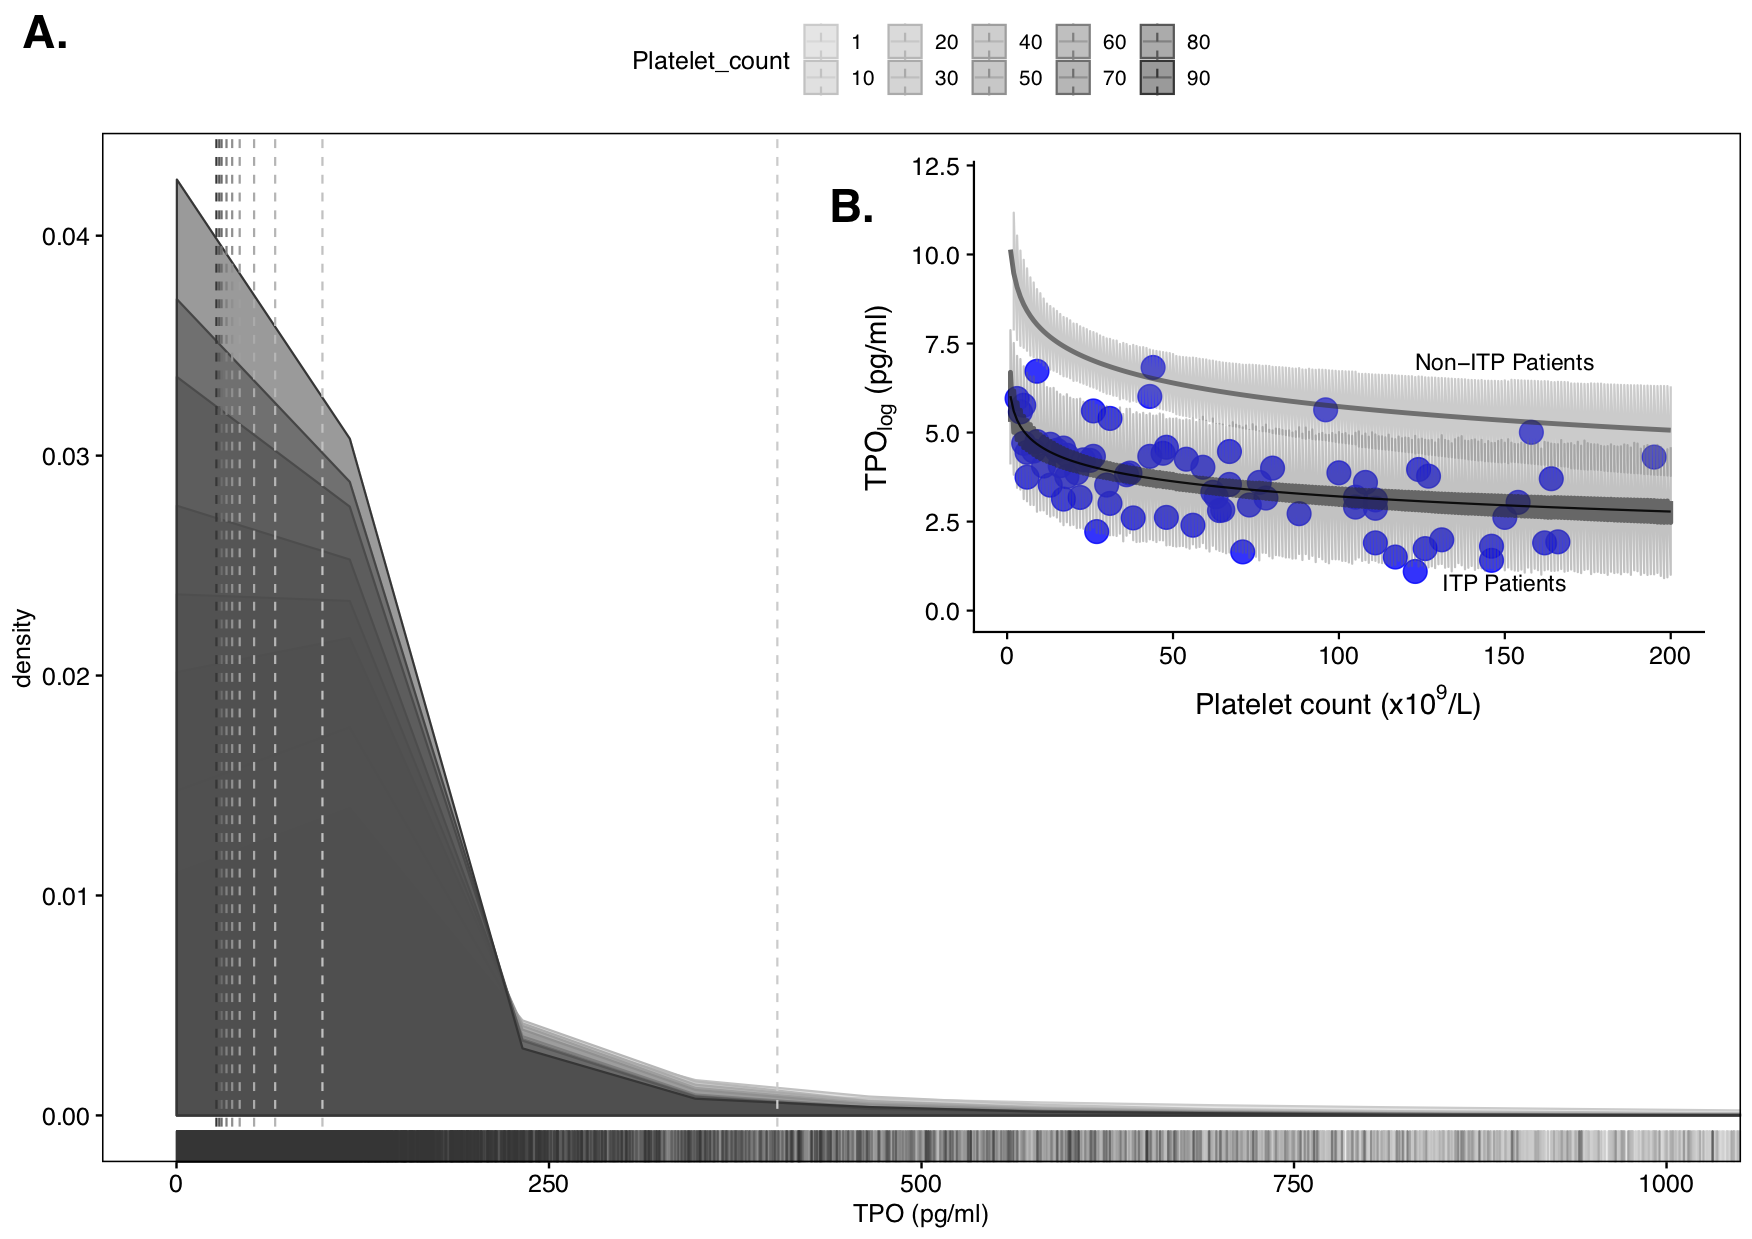
\includegraphics[]{ABSTRACT_v3_graph1.png}
\caption{FIGURE 1: A.) Shows predicted TPO distributions for at different platelet counts ranging from 1 to 90 in our ITP patient group. Dashed vertical lines represent MAP estimates for each distribution. B.) lines shows model predictions for LogTPO levels versus platelet counts in both ITP patients (lower line) and Aplastic controls (upper line).  showing individual patient results and the predicted non-linear assocaition produced by model. Darker shaded area is the 90\% bayesian confidence interval and the lighter shaded area around curve shows total predicted distribution width}
\end{figure}

\bibliographystyle{plain}
\bibliography{tpobib.bib}


\paragraph{}
\textbf{Currently 4504 characters - needs to be characters: 3800}


\end{document}
